\documentclass[review]{elsarticle}

\usepackage{amsmath,amssymb}
\usepackage{booktabs}
\usepackage{graphicx}
\usepackage{lineno}
\usepackage{hyperref}
\usepackage{wasysym}
\usepackage{placeins}
\usepackage{float}

\journal{Measurement}
\biboptions{sort&compress}
\bibliographystyle{elsarticle-num}

\begin{document}

\begin{frontmatter}
\title{Supplementary Materials: Banach-Space Norm Descriptors for Interferometric Profile Metrology}
\end{frontmatter}

\section{Supplementary Experimental Details}

\subsection{Rotation stage specifications}

\begin{table}[H]
\centering
\caption{Technical specifications of the rotation stage~\cite{NewportCorporation:2018vk}.}
\label{tab:supp_stage_spec}
\begin{tabular}{ll}
\toprule
Parameter & Specification \\
\midrule
Angular range & Unrestricted number of revolutions \\
Maximum speed & $80^\circ$/s \\
Encoder accuracy & 2.0 mdeg \\
Wobble, typical & $\pm 12$ $\mu$rad \\
Wobble, guaranteed & $\pm 25$ $\mu$rad \\
Eccentricity, typical & $\pm 0.40$ $\mu$m \\
Transversal compliance & 10 $\mu$rad/N m \\
Origin repeatability & $\pm 0.25$ mdeg \\
\bottomrule
\end{tabular}
\end{table}

\subsection{Environmental shielding and vibration isolation}

\begin{figure}[H]
\centering
\begin{minipage}[t]{0.45\textwidth}
\centering
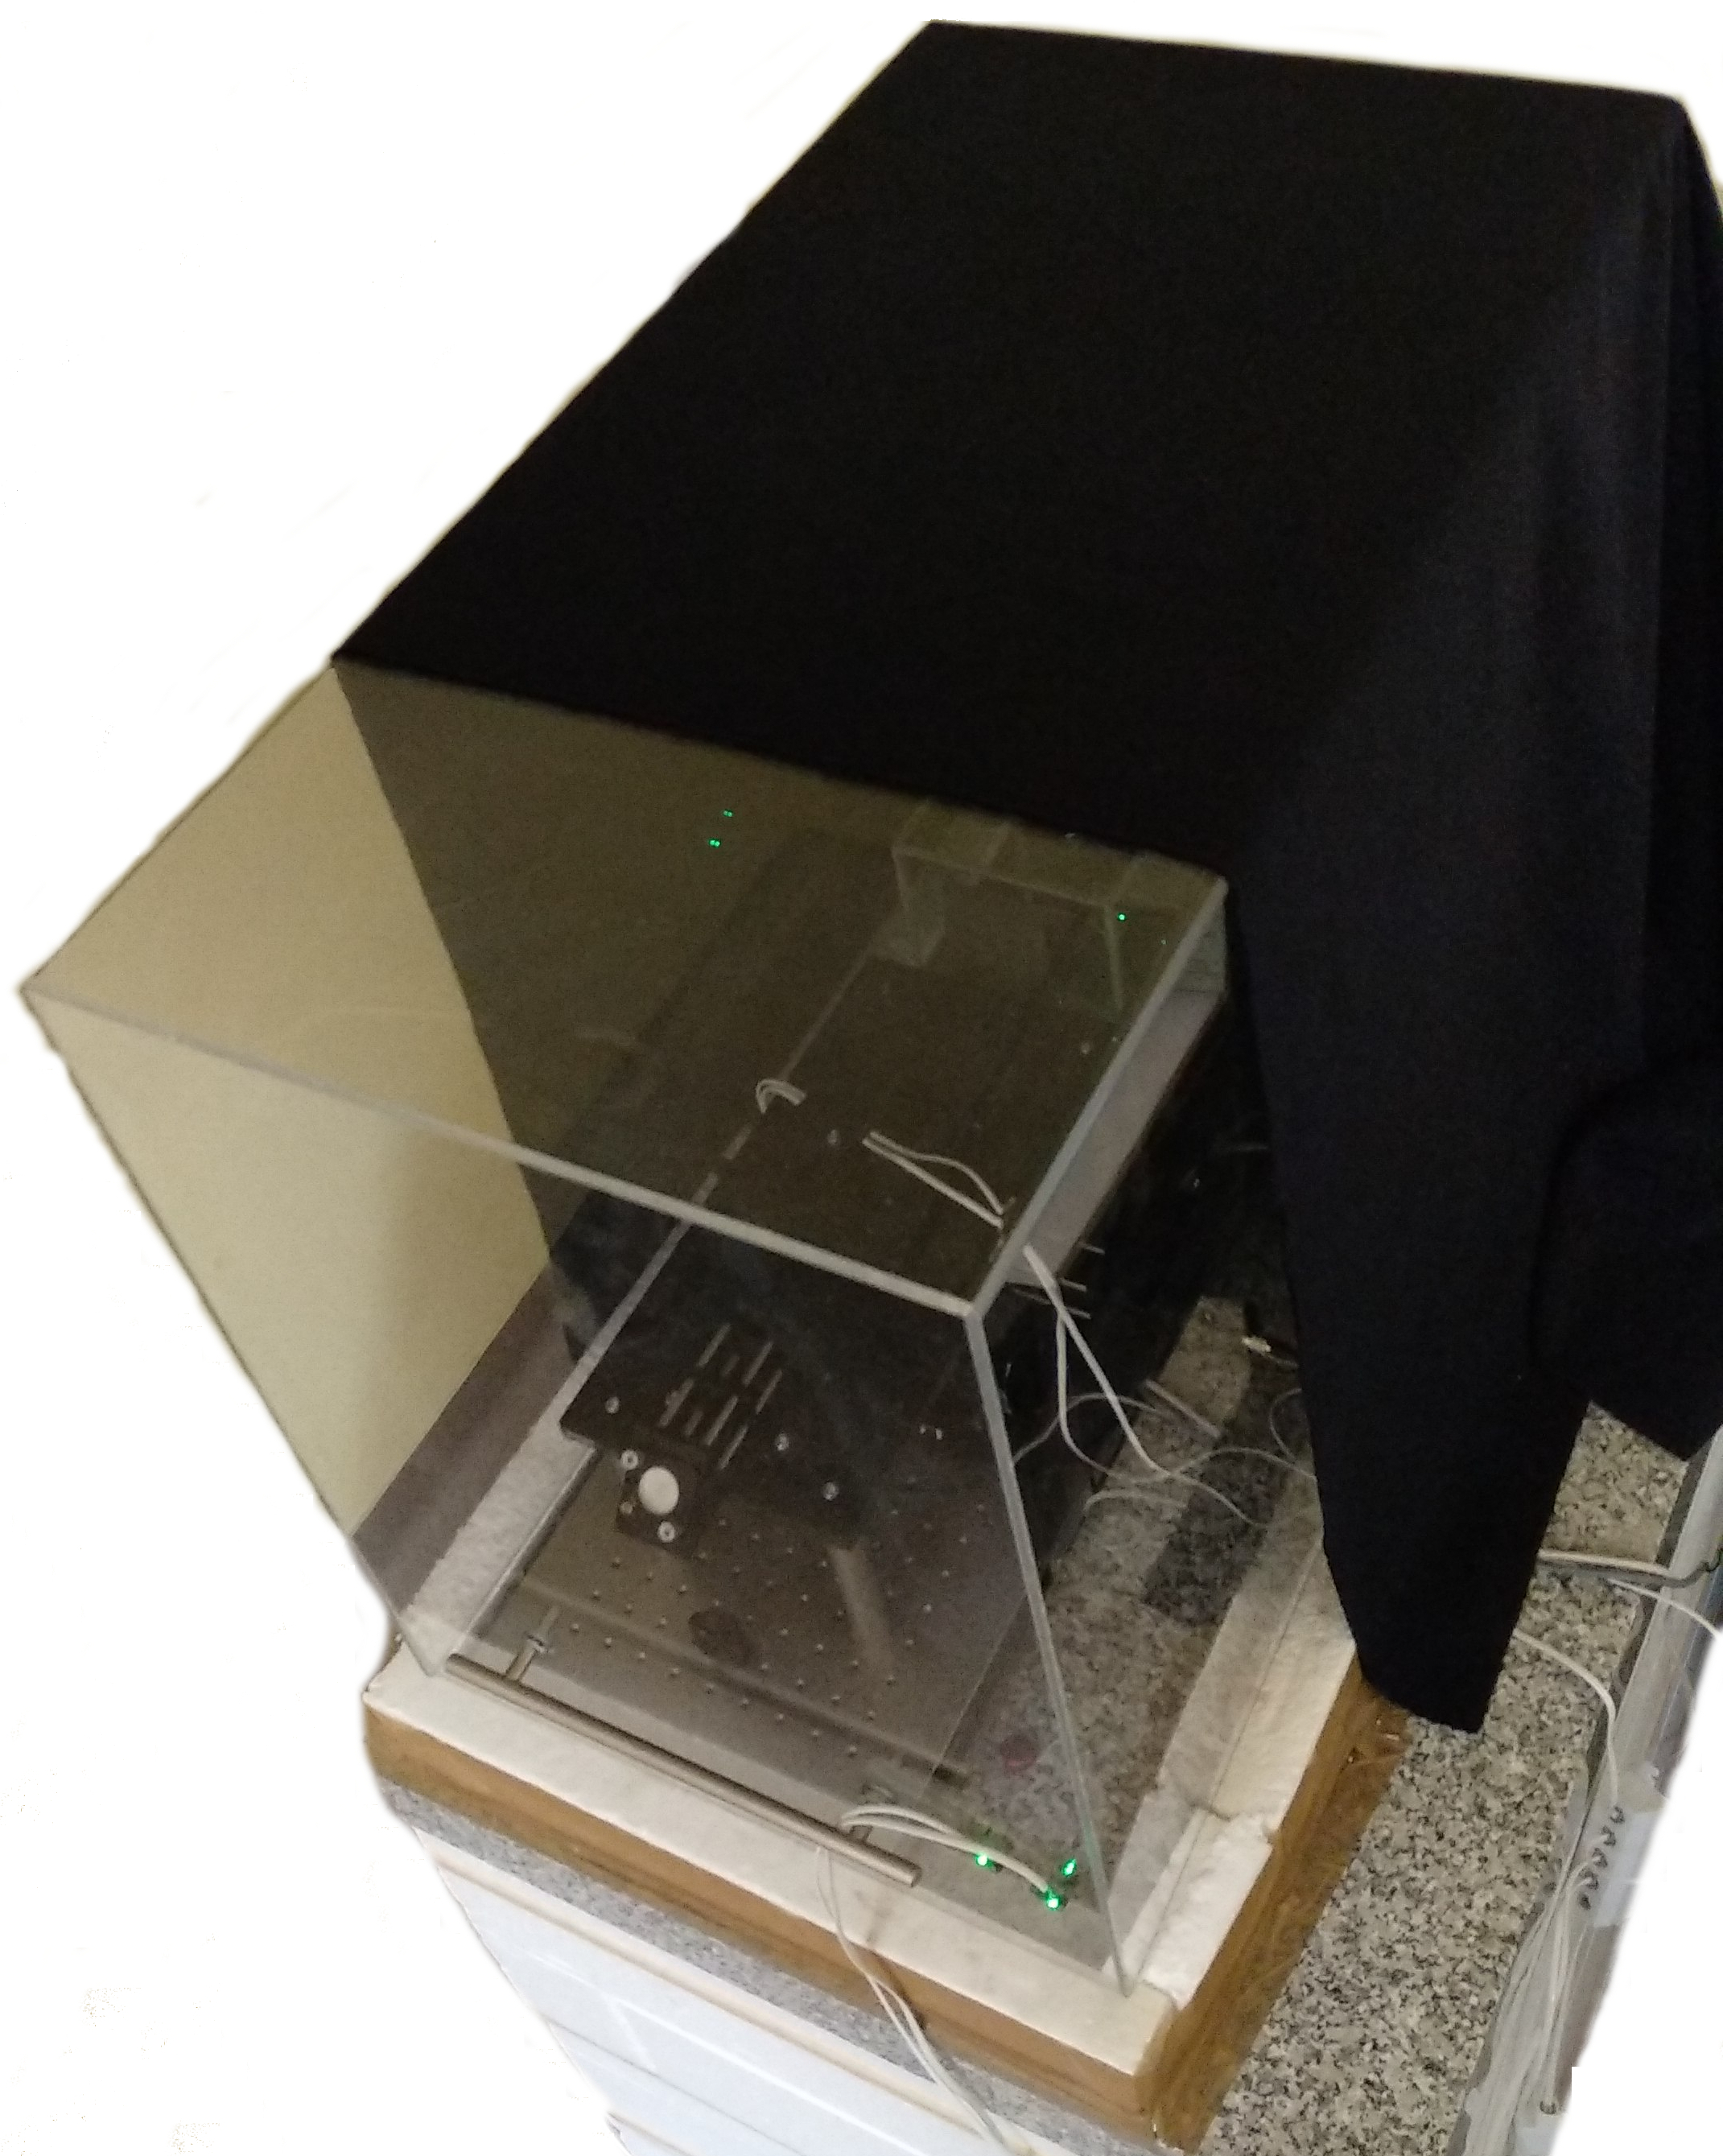
\includegraphics[width=\textwidth]{figs/blanket.jpg}
\caption{Setup shielded by a plexiglass box and covered by a wool blanket.}
\label{fig:supp_blanket}
\end{minipage}
\hfill
\begin{minipage}[t]{0.45\textwidth}
\centering
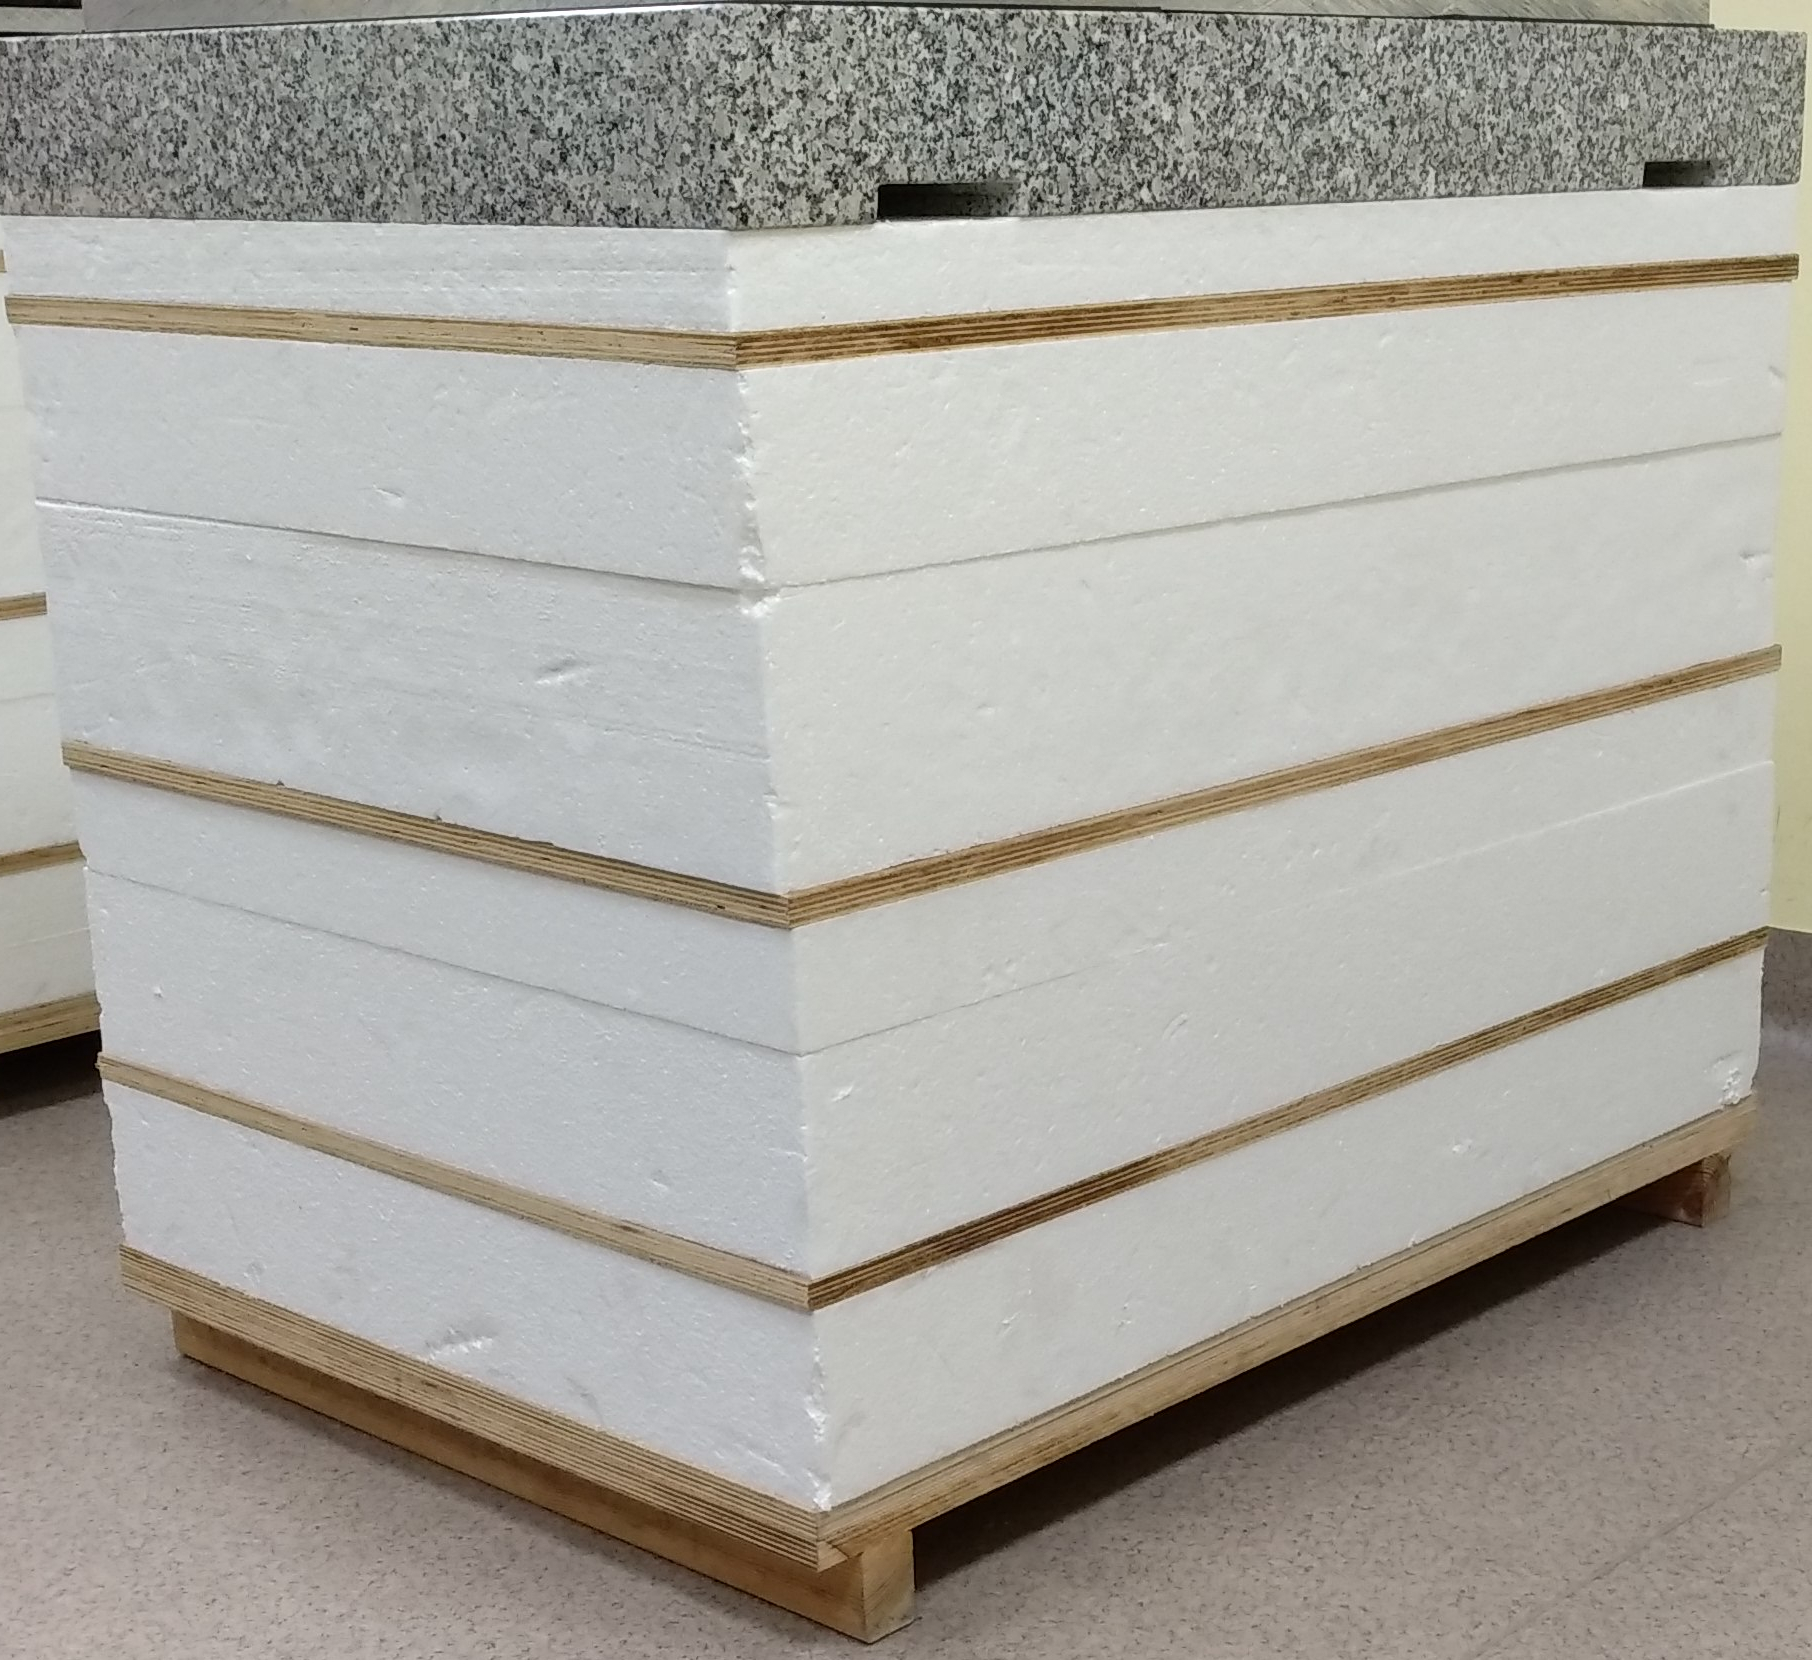
\includegraphics[width=\textwidth]{figs/styrofoam_support.jpg}
\caption{Layered wooden-polystyrene support with granite plate.}
\label{fig:supp_styrofoam}
\end{minipage}
\end{figure}

\subsection{Single-image radial phase extraction}

\begin{figure}[H]
\centering
\includegraphics[width=\textwidth]{../../results/radial_profile_reconstruction_metric/ceramic/radial_phase_extraction.pdf}
\caption{Ceramic single-image radial phase extraction. (Left) Raw interferogram (648$\times$488 px). (Centre) Radial fringe intensity after background subtraction and B-spline smoothing with detected bright-ring maxima marked. (Right) $D_j^2$--order linear fit: the $D^2=0$ intercept (dashed) gives $1-\epsilon$.}
\label{fig:supp_ceramic_radial_phase}
\end{figure}

\begin{figure}[H]
\centering
\includegraphics[width=\textwidth]{../../results/radial_profile_reconstruction_metric/steel/radial_phase_extraction.pdf}
\caption{Steel single-image radial phase extraction. Same EFM procedure applied to a steel interferogram (640$\times$480 px).}
\label{fig:supp_steel_radial_phase}
\end{figure}

\begin{figure}[H]
\centering

\includegraphics[width=\textwidth]{../../results/radial_profile_reconstruction_metric/ceramic/phase_processing_steps.pdf}
\caption{Ceramic sequence processing. (Top left) Wrapped excess fraction. (Top right) Unwrapped fringe order. (Bottom left) Nanometre height profile with LSCI reference circle and eccentricity fit. (Bottom right) Gaussian low-pass filtered residual (50\% at 15~UPR, ISO~16610-21).}
\label{fig:supp_ceramic_phase_steps}
\end{figure}

\begin{figure}[H]
\centering

\includegraphics[width=\textwidth]{../../results/radial_profile_reconstruction_metric/steel/phase_processing_steps.pdf}
\caption{Steel sequence processing. (Top left) Wrapped excess fraction. (Top right) Unwrapped fringe order with linear drift. (Bottom left) Nanometre height profile after detrending. (Bottom right) Gaussian low-pass filtered residual.}
\label{fig:supp_steel_phase_steps}
\end{figure}

\section{Supplementary Validation Analyses}

\FloatBarrier
\subsection{Descriptor comparison and uncertainty}

\begin{figure}[H]
\centering
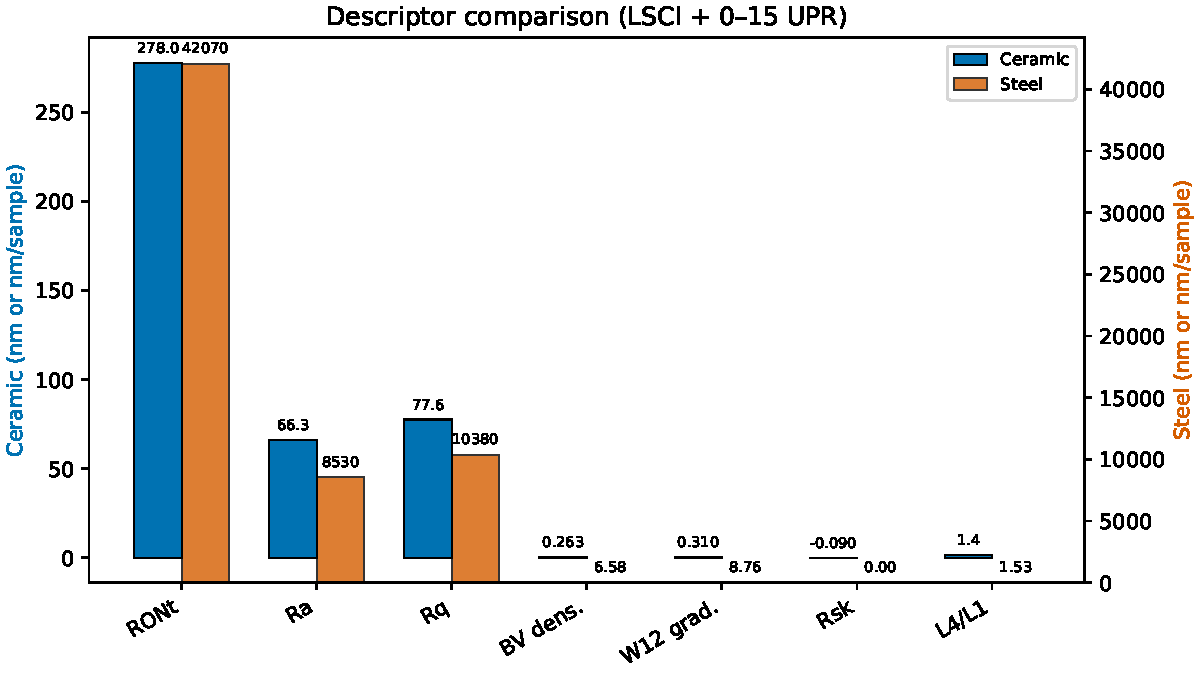
\includegraphics[width=0.95\textwidth]{../../results/radial_profile_reconstruction_metric/sample_comparison_metrics.pdf}
\caption{Comparison of ISO and gradient-based descriptors for both artefacts (bar charts). FN~111 and FN~101 values shown side by side. Error bars: 95\% expanded within-run repeatability ($n=5$).}
\label{fig:supp_metric_comparison}
\end{figure}

\begin{figure}[H]
\centering
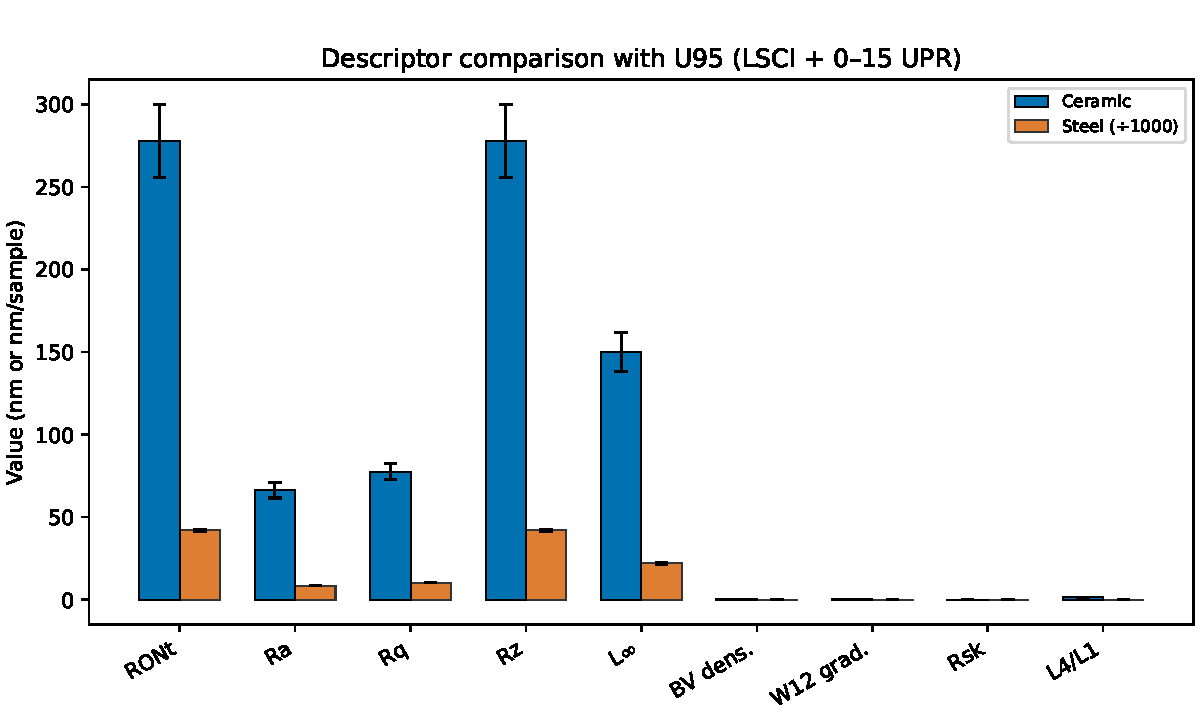
\includegraphics[width=0.95\textwidth]{../../results/radial_profile_reconstruction_metric/iso_banach_uncertainty_table.pdf}
\caption{Uncertainty comparison: relative expanded uncertainty for each descriptor, colour-coded by descriptor family (ISO/profile vs.\ Banach/gradient), for both artefacts.}
\label{fig:supp_uncertainty}
\end{figure}

\FloatBarrier
\subsection{Descriptor independence validation}

\begin{figure}[H]
\centering
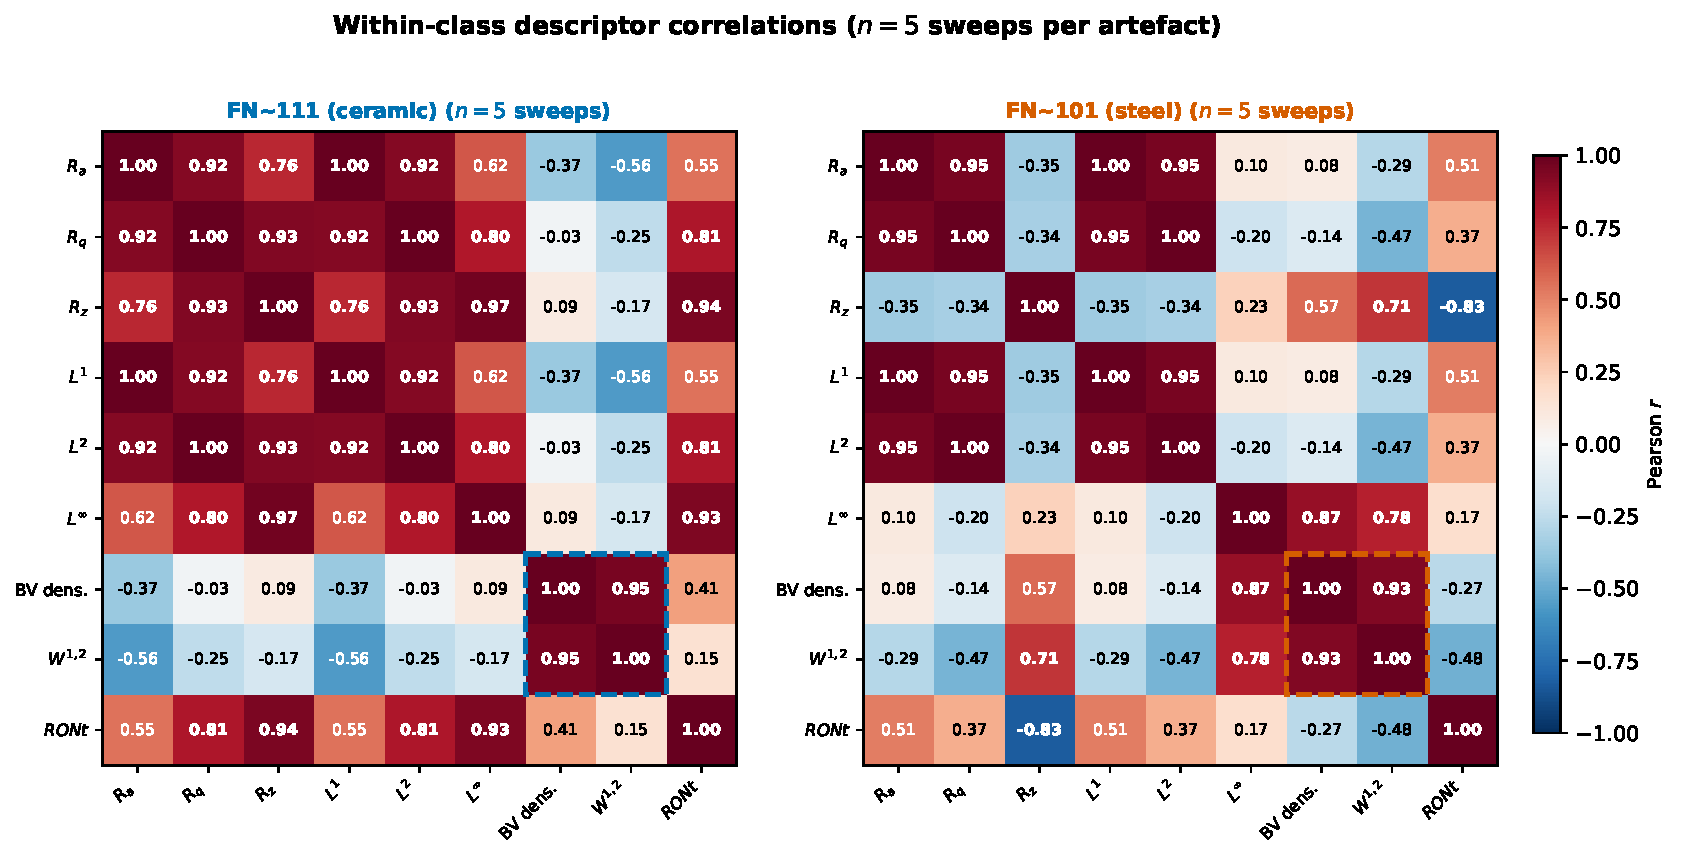
\includegraphics[width=\textwidth]{../../results/radial_profile_reconstruction_metric/descriptor_correlation_heatmap.pdf}
\caption{Within-class descriptor correlation matrices for FN~111 (left) and FN~101 (right). Dashed boxes highlight the Banach gradient-structure block.}
\label{fig:supp_correlation}
\end{figure}

\begin{figure}[H]
\centering
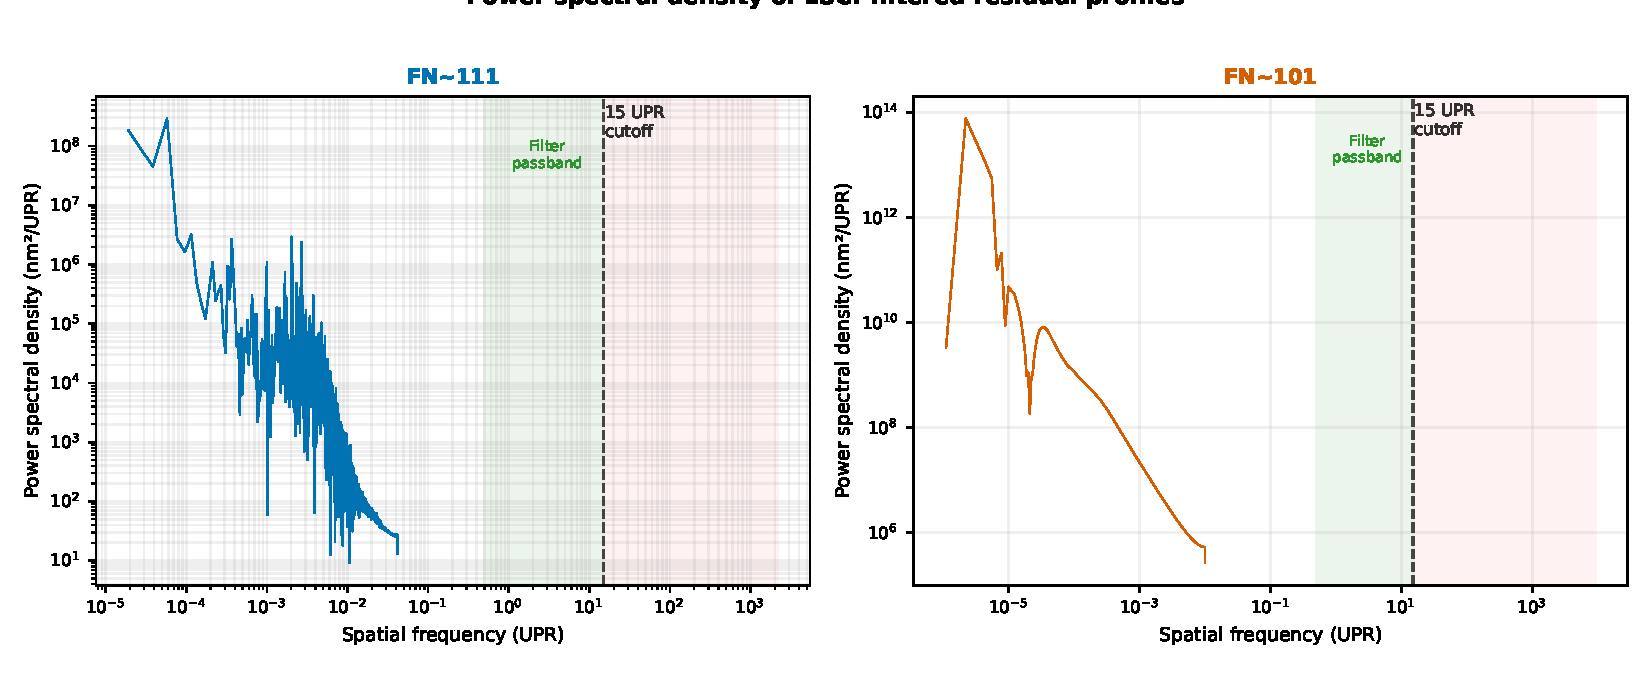
\includegraphics[width=\textwidth]{../../results/radial_profile_reconstruction_metric/profile_psd_comparison.pdf}
\caption{Power spectral density of LSCI-filtered residual profiles (sweep~0). Shaded region: Gaussian filter passband (0.5--15~UPR).}
\label{fig:supp_psd}
\end{figure}

\begin{figure}[H]
\centering
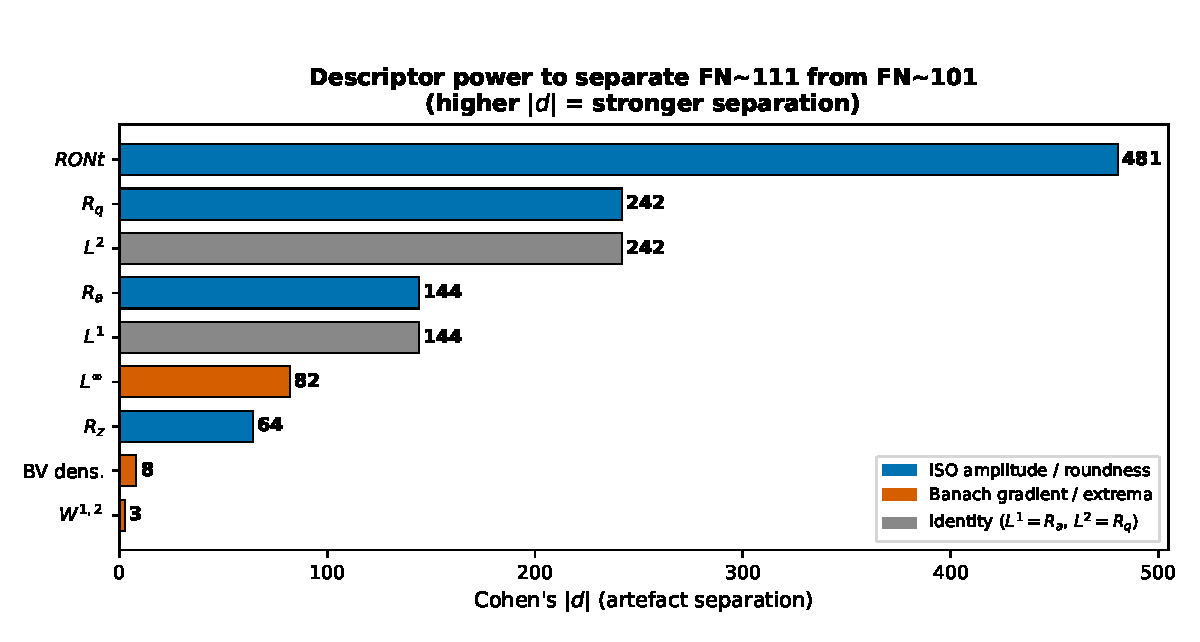
\includegraphics[width=\textwidth]{../../results/radial_profile_reconstruction_metric/cohens_d_artefact_separation.pdf}
\caption{Cohen's $|d|$ effect size for separating FN~111 from FN~101. ISO amplitude/roundness descriptors compared with Banach gradient/extremum descriptors.}
\label{fig:supp_cohens_d}
\end{figure}

\FloatBarrier
\subsection{Critical descriptor assessment}

\begin{figure}[H]
\centering
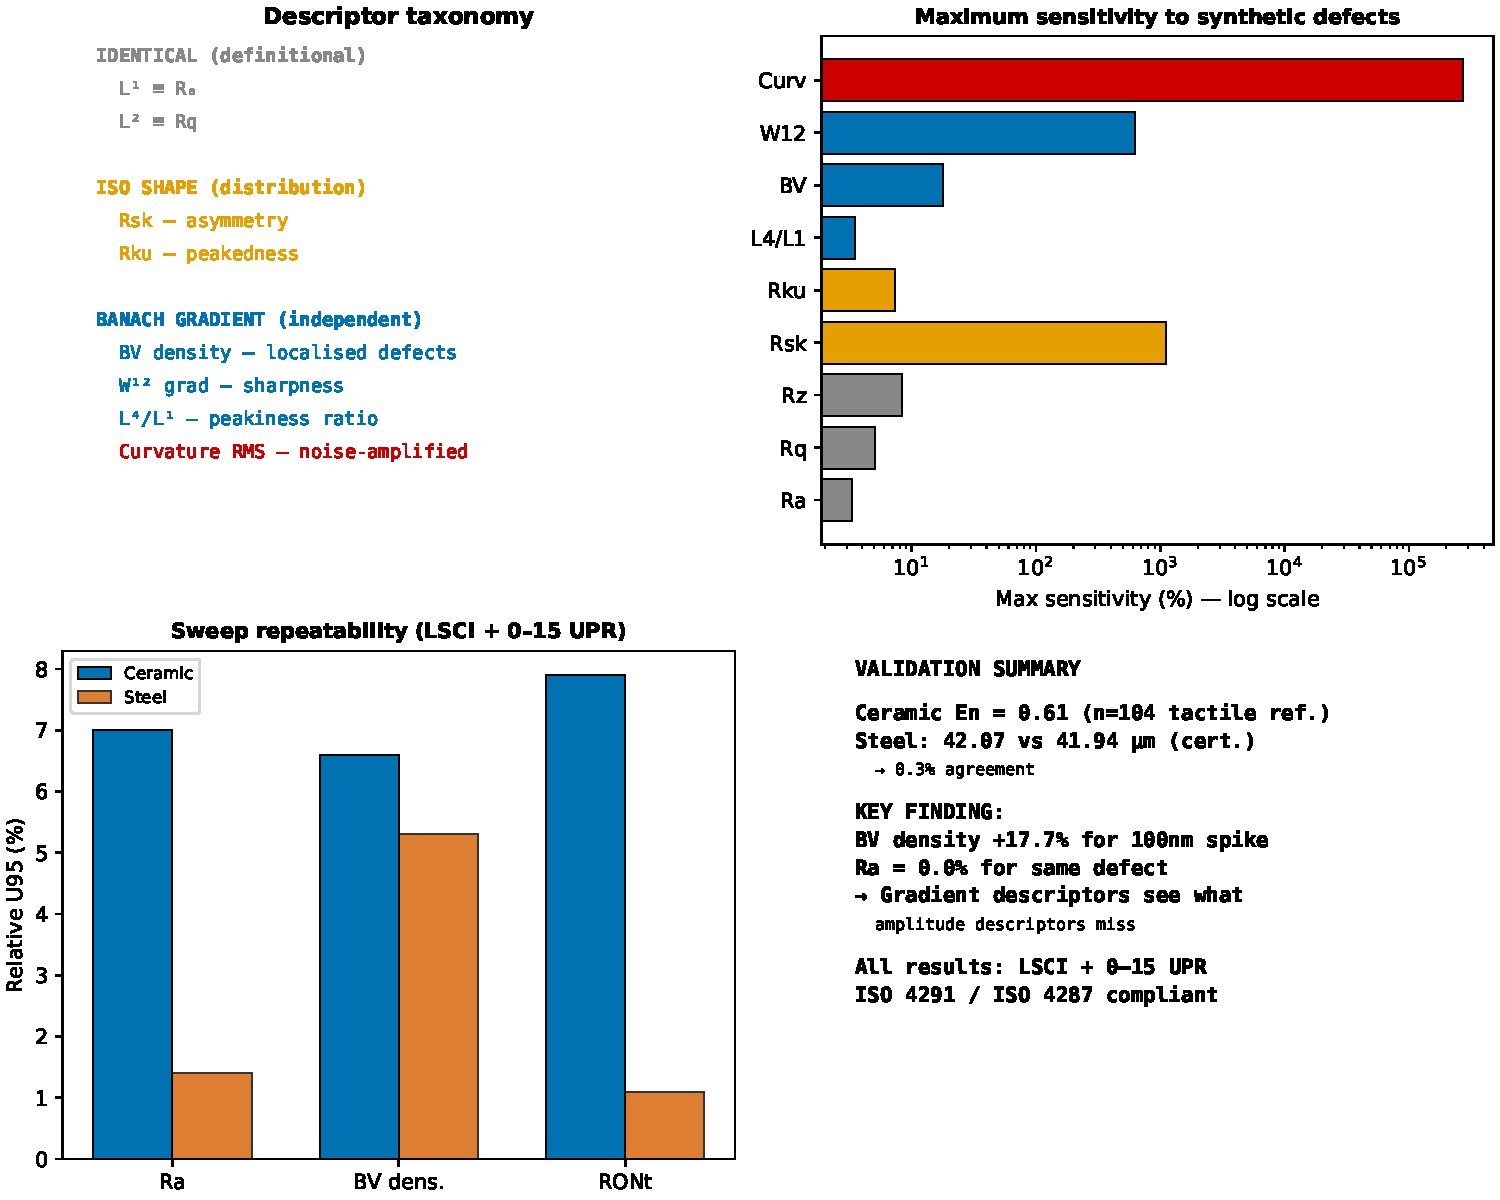
\includegraphics[width=\textwidth]{../../results/radial_profile_reconstruction_metric/banach_iso_critical_comparison.pdf}
\caption{Critical assessment of gradient-based versus ISO descriptors. (Top left) Descriptor taxonomy. (Top right) Maximum sensitivity to synthetic defects. (Bottom left) Sweep-to-sweep stability. (Bottom right) Information-content summary.}
\label{fig:supp_critical}
\end{figure}

\begin{figure}[H]
\centering
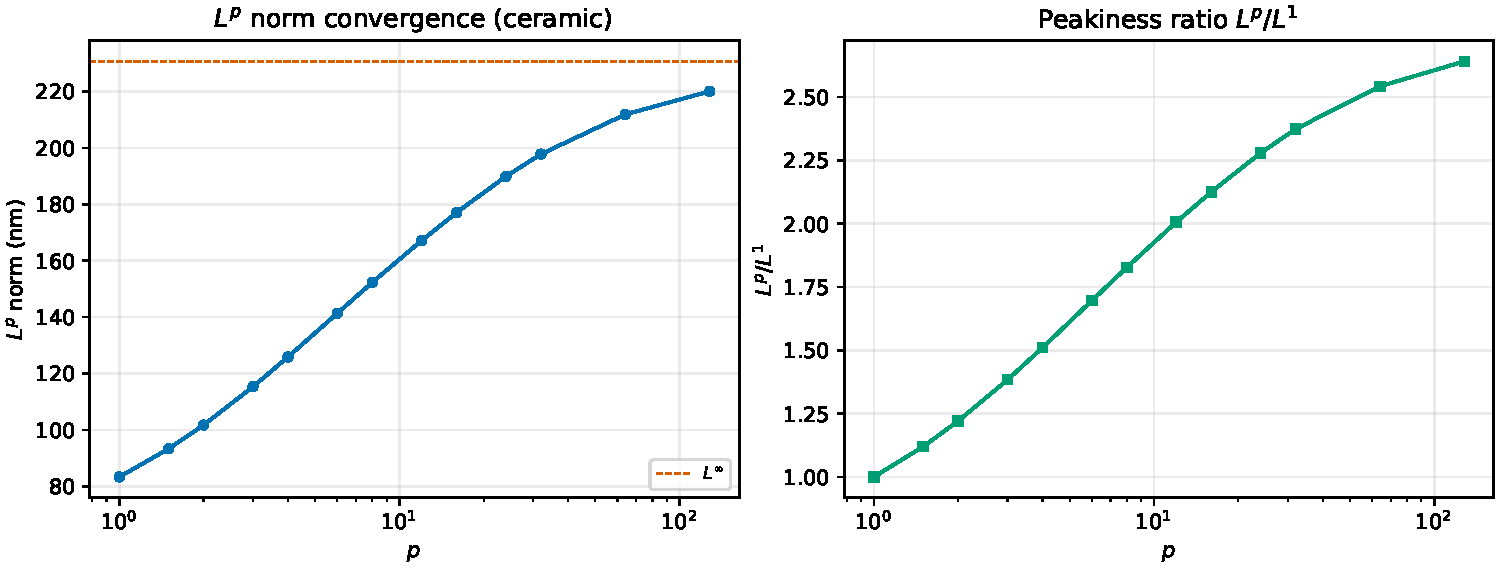
\includegraphics[width=0.9\textwidth]{../../results/radial_profile_reconstruction_metric/lp_convergence.pdf}
\caption{$L^p$ norm convergence for the FN~111 residual profile (unfiltered). (Left) $L^p$ as a function of $p$. (Right) Peakiness ratio $L^p/L^1$.}
\label{fig:supp_lp_convergence}
\end{figure}

\FloatBarrier
\section{Supplementary Sensitivity and Artefact-Specific Analyses}

\subsection{Descriptor sensitivity to synthetic defects}

\begin{table}[H]
\centering
\small
\caption{Sensitivity of ISO and gradient-based descriptors to synthetic profile defects. Values are percentage change from the unperturbed ceramic baseline (LSCI + Gaussian low-pass, 50\% at 15~UPR; $R_a=61.9$~nm, $R_q=71.0$~nm). Bold entries indicate changes exceeding 10\%. Defect details: Spike = single $100$~nm point; Scratch = $5\times50$~nm depression; Waviness = $20$~nm sinusoid ($\lambda=500$ samples); Step = $30$~nm offset; Noise = $5$~nm RMS white noise.}
\label{tab:supp_descriptor_sensitivity}
\begin{tabular}{lccccc}
\toprule
Descriptor & Spike & Scratch & Waviness & Step & Noise \\
\midrule
\multicolumn{6}{c}{\textit{Amplitude-averaging ISO parameters}} \\
$R_a$ & $-$0.0\% & $+$0.1\% & $+$3.2\% & $+$3.3\% & $+$0.1\% \\
$R_q$ & $-$0.0\% & $+$0.1\% & $+$3.3\% & $+$5.1\% & $+$0.2\% \\
$R_z$ (PV) & $+$0.0\% & $+$0.0\% & $+$7.0\% & $-$2.6\% & $+$8.4\% \\
\multicolumn{6}{c}{\textit{ISO shape parameters}} \\
$R_{sk}$ (skewness) & $-$0.4\% & $+$6.7\% & \textbf{$-$168.5\%} & \textbf{$-$1103.7\%} & $-$0.1\% \\
$R_{ku}$ (kurtosis) & $+$0.0\% & $+$0.1\% & $+$2.4\% & $+$7.3\% & $+$0.4\% \\
\multicolumn{6}{c}{\textit{Gradient-structure descriptors}} \\
$L^4/L^1$ peakiness & $+$0.0\% & $+$0.0\% & $+$0.7\% & $+$3.5\% & $+$0.2\% \\
$BV$ density & \textbf{$+$17.7\%} & $+$8.9\% & \textbf{$+$11.7\%} & $+$2.7\% & \textbf{$+$2077.4\%} \\
$W^{1,2}$ grad.\ seminorm & \textbf{$+$621.8\%} & \textbf{$+$271.2\%} & \textbf{$+$16.9\%} & \textbf{$+$81.7\%} & \textbf{$+$2260.9\%} \\
Curvature RMS & \textbf{$+$273\,161\%} & \textbf{$+$111\,458\%} & \textbf{$+$94\%} & \textbf{$+$47\,230\%} & \textbf{$+$901\,073\%} \\
\bottomrule
\end{tabular}
\end{table}

The results lead to five conclusions:
\begin{enumerate}
  \item Amplitude-averaging ISO descriptors ($R_a$, $R_q$, $R_z$) show negligible sensitivity to localised defects. A single $100$~nm spike changes $R_a$ by $0.0\%$, $R_q$ by $0.0\%$, and $R_z$ by $0.0\%$.
  \item ISO shape parameters respond to asymmetry but not to symmetric localised features. $R_{sk}$ changes by $-1104\%$ for a step defect (strong asymmetry), but only $-0.4\%$ for a symmetric spike. $R_{ku}$ is insensitive to all tested defects.
  \item Gradient-structure descriptors provide substantially higher sensitivity to localised defects than any single ISO~4287 parameter. BV density increases by $+18\%$ for a spike, $+9\%$ for a scratch, and $+12\%$ for waviness. The $W^{1,2}$ gradient seminorm shows even larger relative changes ($+622\%$ for spike, $+271\%$ for scratch).
  \item $R_{sk}$ and BV density are complementary: $R_{sk}$ detects asymmetry, BV density detects localised gradients regardless of symmetry. Their combination provides descriptive sensitivity beyond any single classical parameter.
  \item Curvature RMS is extremely sensitive to localised defects but strongly sampling-dependent; it should be used only for same-instrument comparisons.
\end{enumerate}

\begin{figure}[H]
\centering
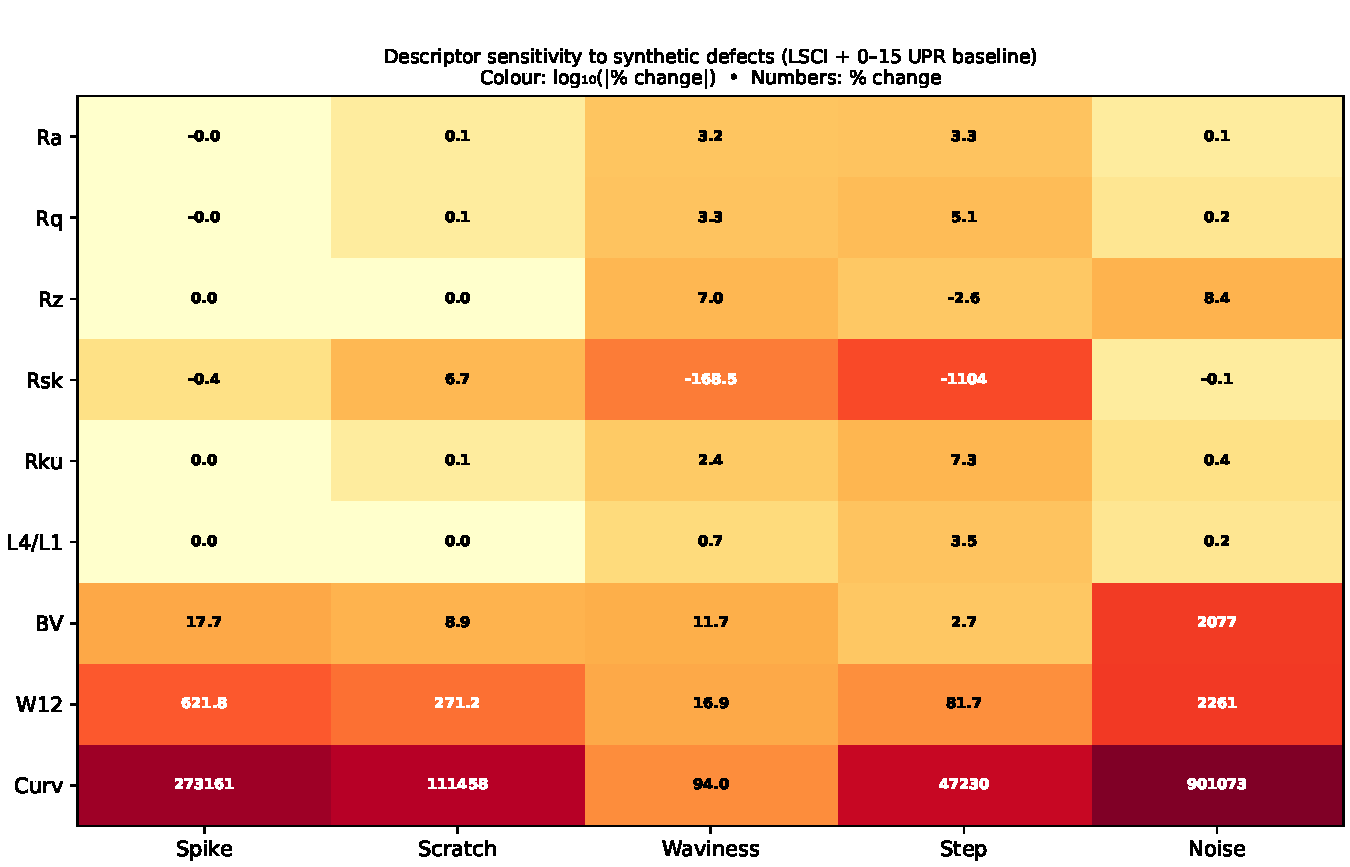
\includegraphics[width=0.95\textwidth]{../../results/radial_profile_reconstruction_metric/descriptor_sensitivity.pdf}
\caption{Sensitivity of ISO and gradient-based descriptors to five synthetic defect types injected into the FN~111 residual profile. Values are percentage change from the unperturbed baseline. Bold labels indicate changes exceeding 10\%.}
\label{fig:supp_descriptor_sensitivity}
\end{figure}

\FloatBarrier
\subsection{Flick flat detection and measurement (FN~101)}

\begin{figure}[H]
\centering
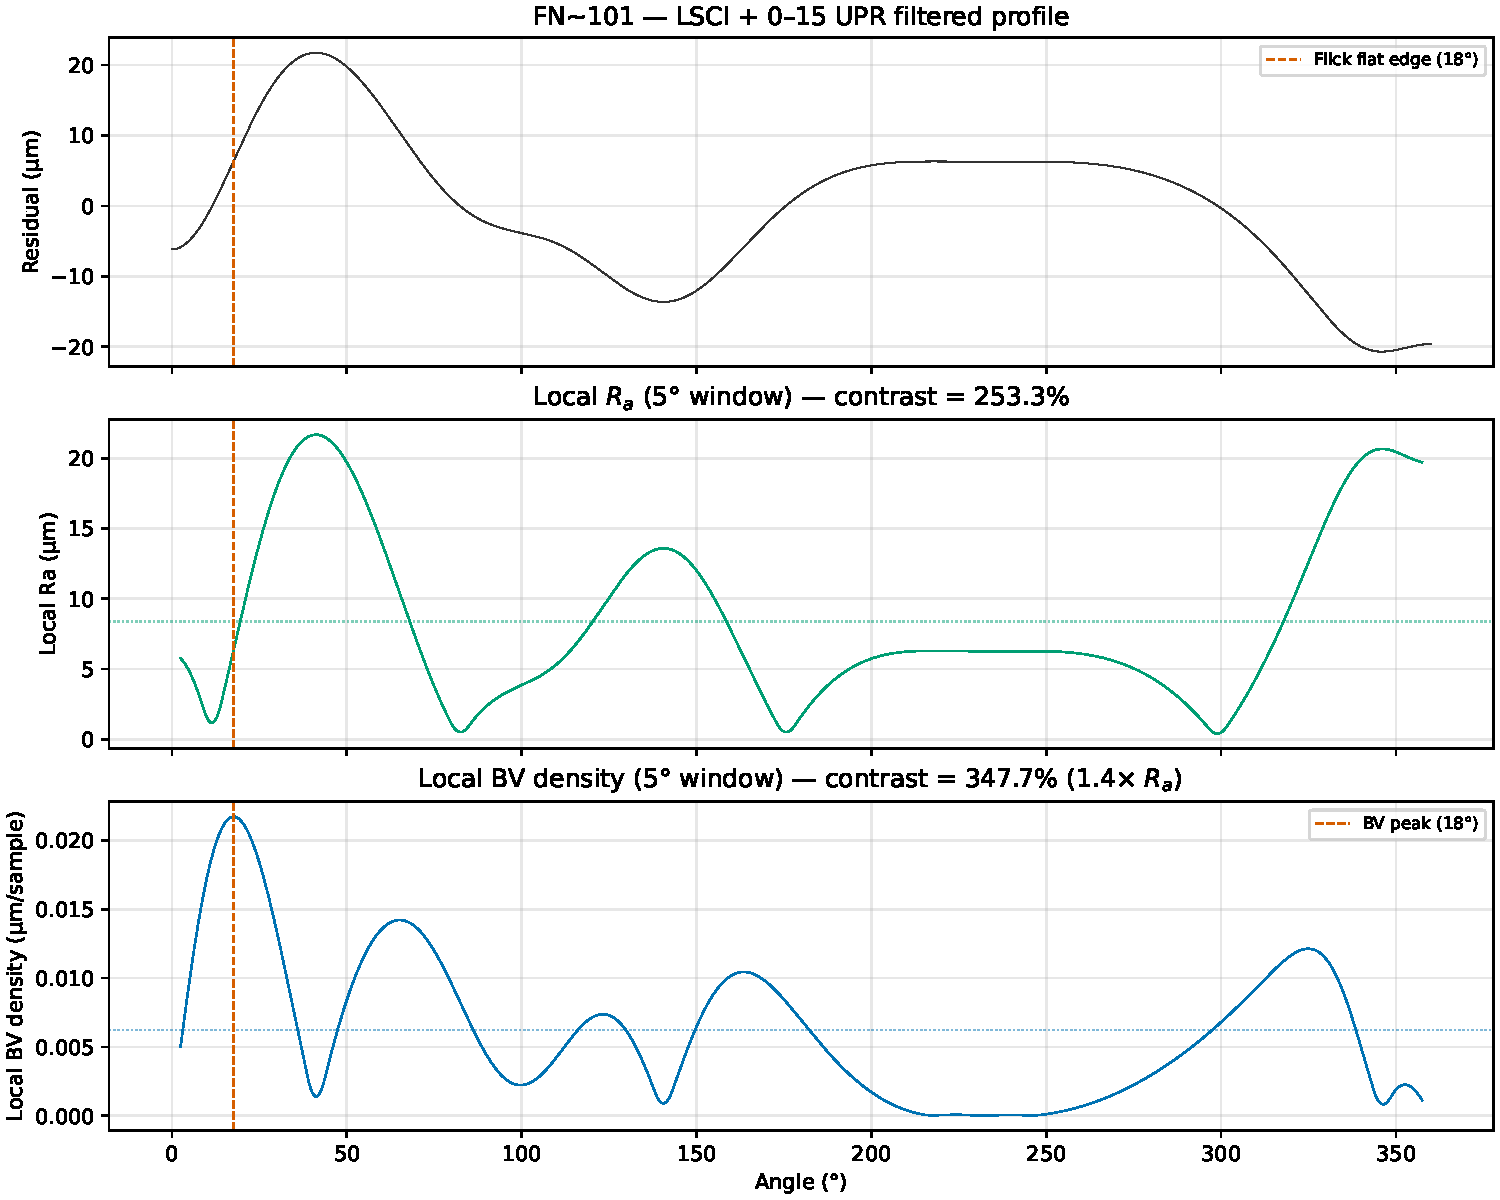
\includegraphics[width=\textwidth]{../../results/radial_profile_reconstruction_metric/flick_flat_detection.pdf}
\caption{Flick flat detection on the JENOPTIK magnification standard FN~101. BV density (bottom panel) shows a clear spike at the Flick flat angular position, whereas the ISO~4287 amplitude parameter $R_a$ (computed in a sliding window, top panel) shows negligible response. This demonstrates the complementary gradient-sensitive information provided by BV density beyond amplitude averaging.}
\label{fig:supp_flick_flat_detection}
\end{figure}

\begin{figure}[H]
\centering
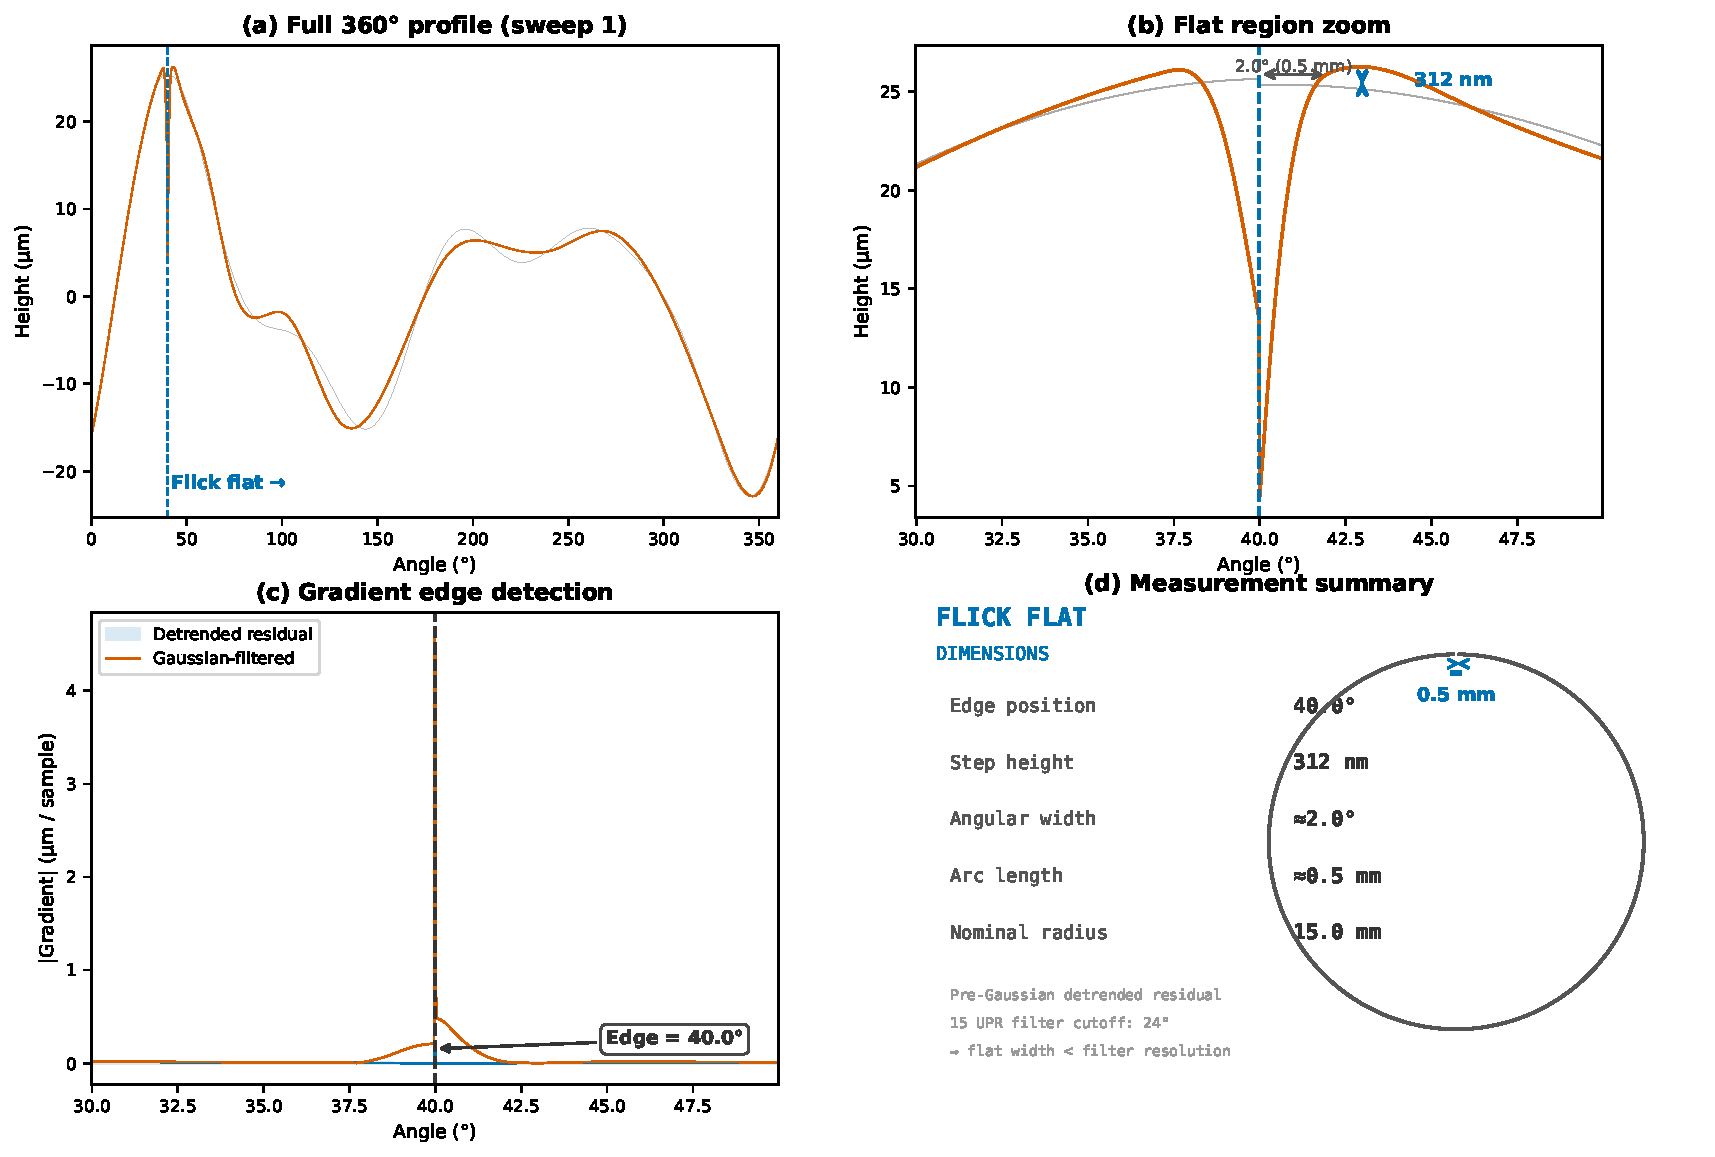
\includegraphics[width=\textwidth]{../../results/radial_profile_reconstruction_metric/flick_flat_measurement.pdf}
\caption{Flick flat measurement on the JENOPTIK magnification standard FN~101. Reconstructed profile across the Flick flat sector showing the characteristic step-like geometry, with the flat region and adjacent roundness profile labelled. $RONt = 42.07~\mu$m is dominated by the Flick flat depth.}
\label{fig:supp_flick_flat_measurement}
\end{figure}

\FloatBarrier
\subsection{Cross-instrument validation: optical versus tactile}

\begin{figure}[H]
\centering
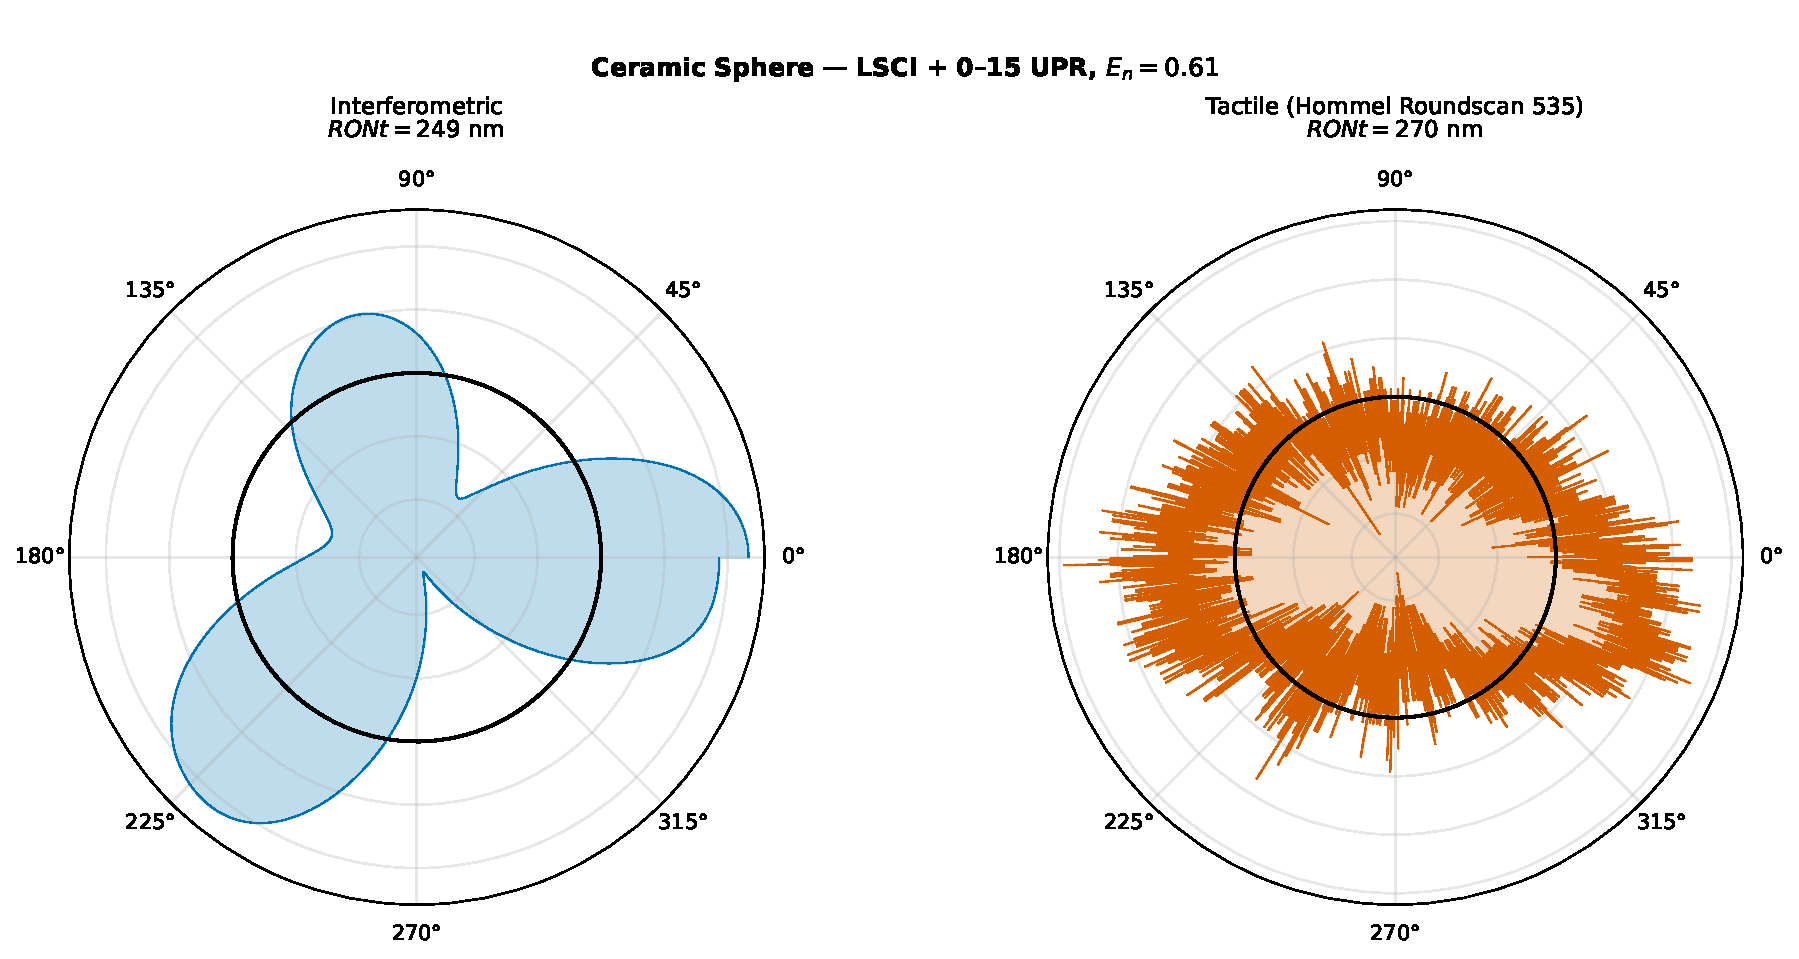
\includegraphics[width=\textwidth]{../../results/radial_profile_reconstruction_metric/ceramic_tactile_comparison_polar.pdf}
\caption{Polar comparison of optical (this work) and tactile reference (Hommel Roundscan~535) roundness profiles for the FN~111 standard. Both profiles are LSCI-centred and Gaussian low-pass filtered (50\% at 15~UPR). The optical profile agrees with the tactile reference to within the combined uncertainty ($E_n = 0.61$).}
\label{fig:supp_tactile_comparison}
\end{figure}

\FloatBarrier
\section{Supplementary Artefact Documentation}

\subsection{Artefact photographs}

\begin{figure}[H]
\centering
\begin{minipage}[t]{0.48\textwidth}
\centering
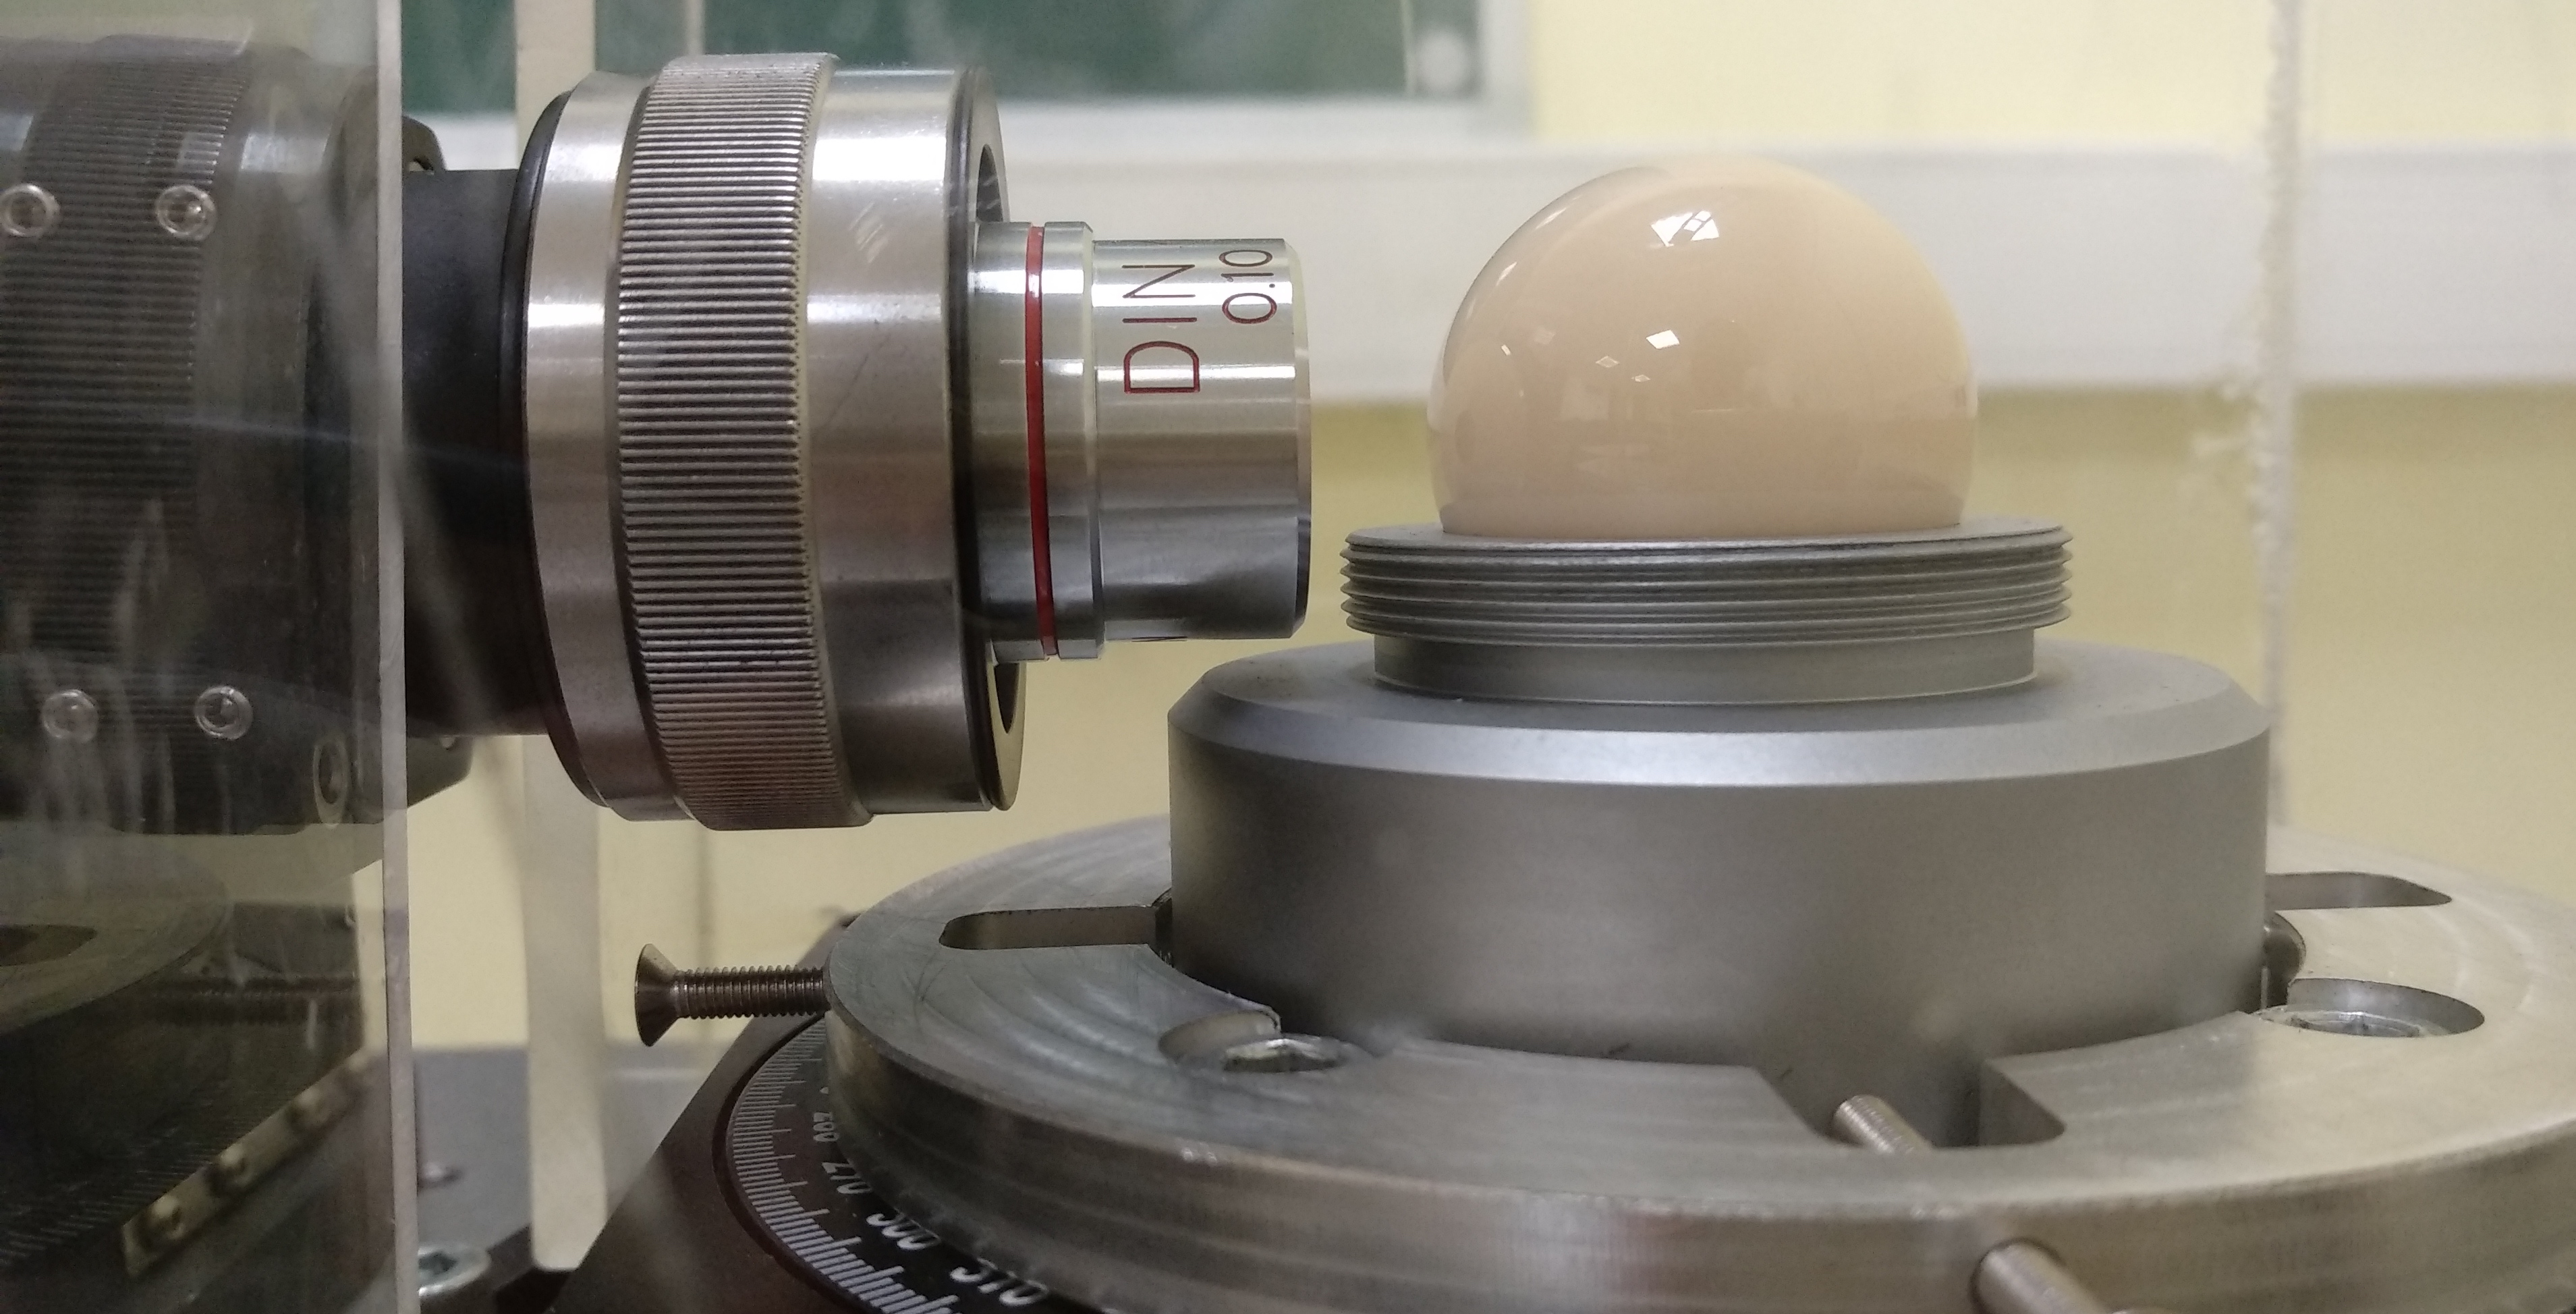
\includegraphics[width=\linewidth]{figs/ceramic_standard.jpg}
\caption{JENOPTIK roundness standard FN~111 ($Al_{2}O_{3}$, $\phi = 29.9588~\mathrm{mm}$). Test report Art.~521~799. DAkkS-DKD calibration certificate Art.~532~529.}
\label{fig:supp_ceramic_standard}
\end{minipage}\hfill
\begin{minipage}[t]{0.48\textwidth}
\centering
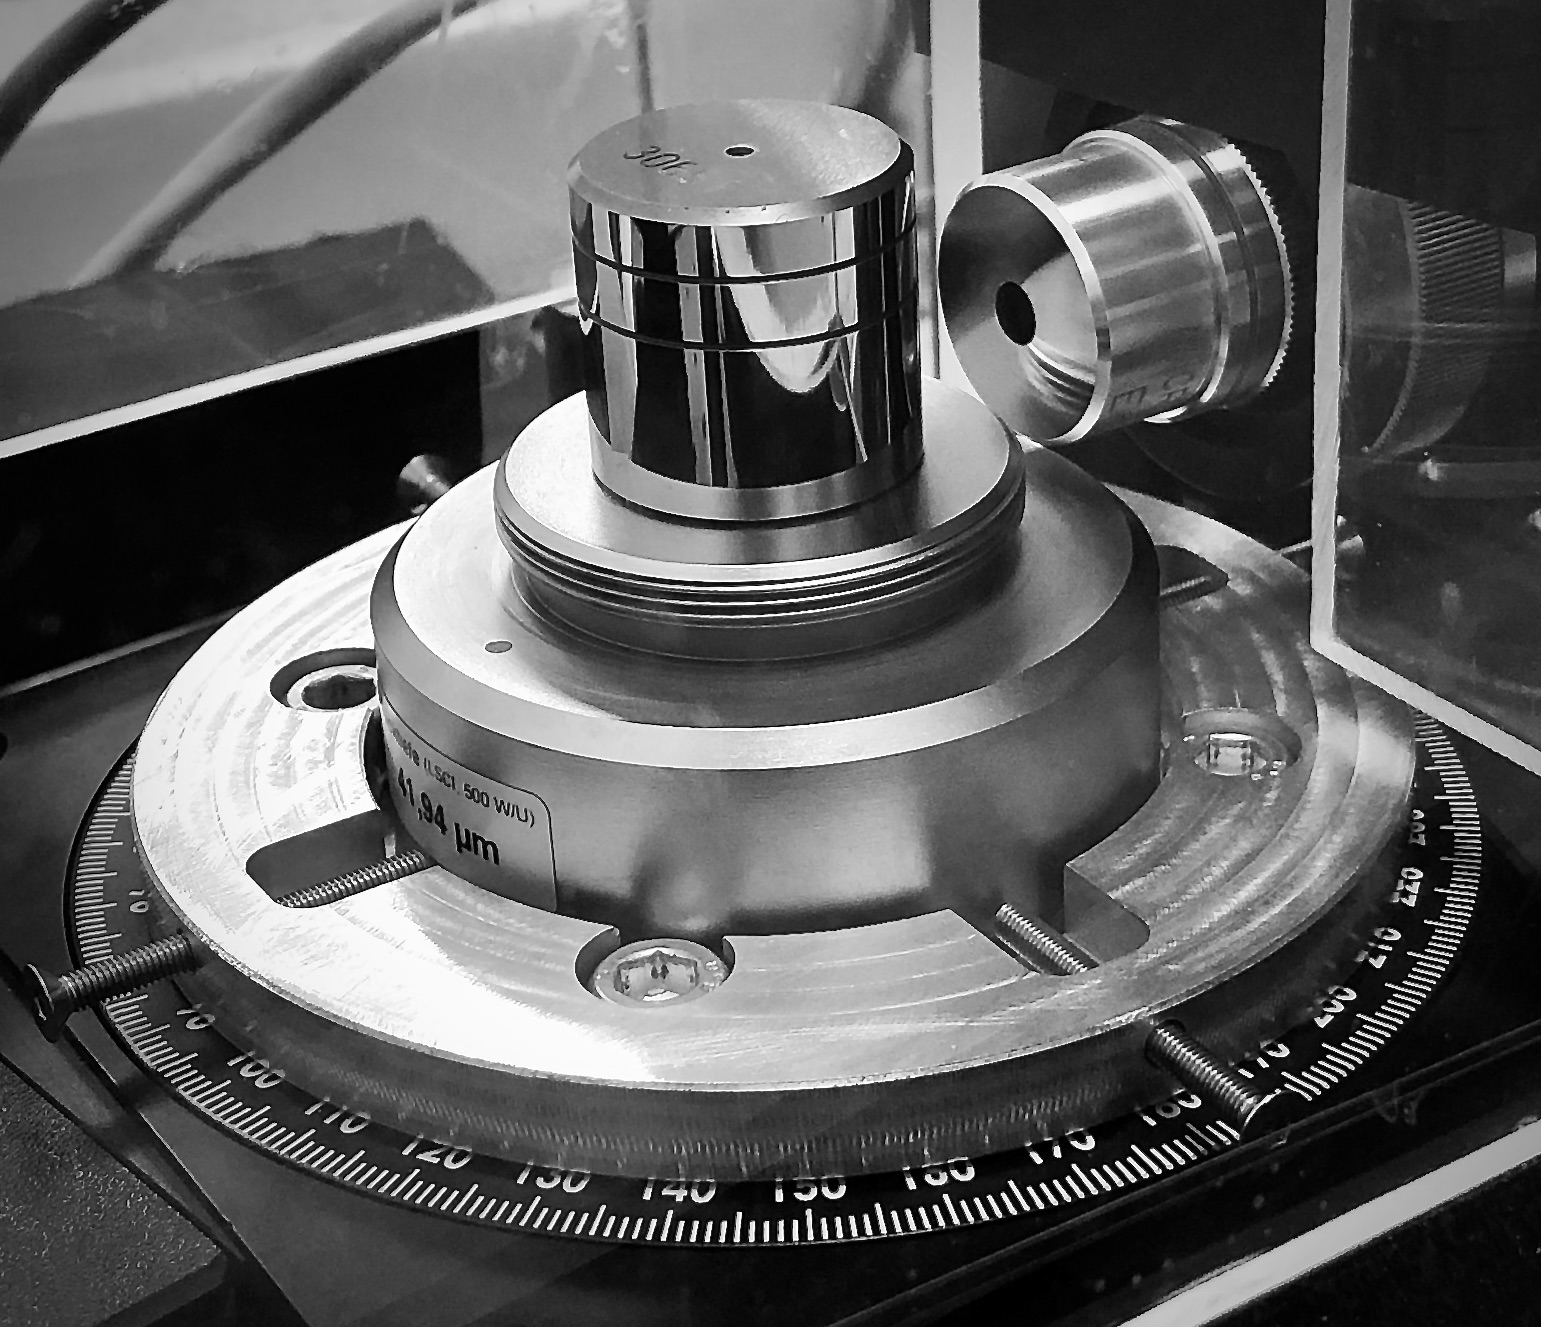
\includegraphics[width=\linewidth]{figs/steel_standard.jpg}
\caption{JENOPTIK magnification standard FN~101. Test report Art.~521~809. DAkkS-DKD calibration certificate Art.~532~528.}
\label{fig:supp_steel_standard}
\end{minipage}
\end{figure}

\subsection{Steel roundness — polar representation (FN~101, Flick flat)}

\begin{figure}[H]
\centering
\includegraphics[width=\textwidth]{../../results/radial_profile_reconstruction_metric/steel/roundness_polar.pdf}
\caption{Steel roundness in polar coordinates (LSCI + Gaussian low-pass, 50\% at 15~UPR). Five sweeps at native angular positions. The Flick flat appears at a shifted angular position in each sweep due to the $40^\circ$ offset between successive $360^\circ$ segments. $RONt = 42.07 \pm 0.48~\mu$m.}
\label{fig:supp_steel_roundness_polar}
\end{figure}

\subsection{Profile reconstruction plots}

\begin{figure}[H]
\centering
\includegraphics[width=\textwidth]{../../results/radial_profile_reconstruction_metric/ceramic/profile_reconstruction.pdf}
\caption{Ceramic profile reconstruction. (Top left) Raw height profiles from all five sweeps, vertically offset for clarity. (Top right) LSCI-centred residual for sweep~0. (Bottom left) Gaussian low-pass filtered residual (50\% at 15~UPR) with $RONt=278$~nm. (Bottom right) Full-sequence ISO and gradient-based descriptors.}
\label{fig:supp_ceramic_profile_reconstruction}
\end{figure}

\begin{figure}[H]
\centering
\includegraphics[width=\textwidth]{../../results/radial_profile_reconstruction_metric/steel/profile_reconstruction.pdf}
\caption{Steel profile reconstruction. (Top left) Detrended height profiles from all five sweeps, vertically offset. (Top right) LSCI-centred residual for sweep~0. (Bottom left) Gaussian low-pass filtered residual (50\% at 15~UPR) with $RONt=42.07~\mu$m. (Bottom right) Full-sequence ISO and gradient-based descriptors.}
\label{fig:supp_steel_profile_reconstruction}
\end{figure}

\end{document}
